\documentclass[tikz,border=6pt]{standalone}
\usepackage{tikz}
\usetikzlibrary{arrows.meta}
\definecolor{nebula}{HTML}{6366F1}
\definecolor{spark}{HTML}{14B8A6}
\definecolor{ink}{HTML}{334155}
\begin{document}
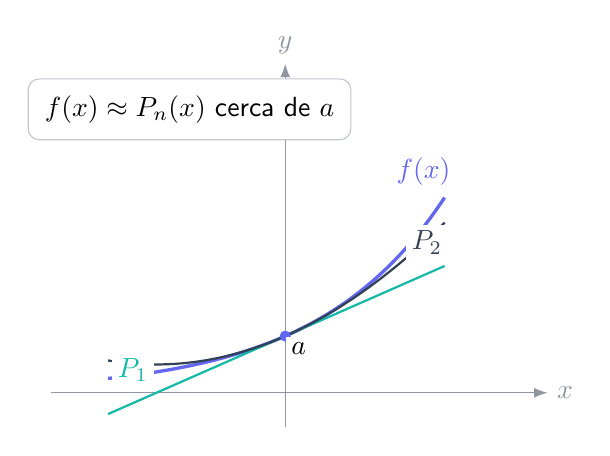
\begin{tikzpicture}[font=\sffamily,>=Latex,x=.9cm,y=.72cm]
  \draw[->,ink!55] (-3.3,0)--(3.7,0) node[right] {$x$};
  \draw[->,ink!55] (0,-.6)--(0,5.8) node[above] {$y$};
  \draw[very thick,nebula,domain=-2.5:2.25,samples=120,smooth] plot(\x,{exp(.55*\x)});
  \draw[thick,spark,domain=-2.5:2.25,samples=2] plot(\x,{1+.55*\x});
  \draw[thick,ink,domain=-2.5:2.25,samples=80] plot(\x,{1+.55*\x+.15125*\x*\x});
  \fill[nebula] (0,1) circle (2pt);
  \node[below right,fill=white,inner sep=2pt] at (0,1) {$a$};
  \node[text=nebula,fill=white,inner sep=2pt] at (1.95,3.9) {$f(x)$};
  \node[text=spark,fill=white,inner sep=2pt] at (-2.15,.4) {$P_1$};
  \node[text=ink,fill=white,inner sep=2pt] at (2.0,2.65) {$P_2$};
  \node[draw=ink!30,rounded corners=4pt,fill=white,inner sep=6pt] at (-1.35,5.0) {$f(x)\approx P_n(x)$ cerca de $a$};
\end{tikzpicture}
\end{document}
